\documentclass[a4paper,10pt]{article}
\usepackage[left=1in, right=1in, top=1in, bottom=1in]{geometry}
\usepackage{enumitem}
\usepackage{graphicx}
\usepackage{tikz}
\usepackage{background}
\usepackage{hyperref}
\usepackage{titlesec}
\usepackage{xcolor}
\usepackage{fancyhdr}
\usepackage{parskip}
\usepackage{tabularx}
\usepackage{multicol}
\usepackage{lipsum} % For dummy text, remove this in your final document

% Define colors
\definecolor{primary}{RGB}{66, 133, 244}
\definecolor{accent}{RGB}{138, 43, 226}
\definecolor{bgcolor}{RGB}{215, 232, 249} % Custom background color

% Background setup
\backgroundsetup{
  scale=3,
  color=bgcolor,
  opacity=0.2,
  angle=0,
  position=current page.south,
  contents={%
    
\begin{tikzpicture}[overlay,remember picture]
      % Diagonal lines
      \draw[color=primary, line width=0.5mm] (0,0) -- (15,10);
      \draw[color=primary, line width=0.5mm] (0,10) -- (15,0);
      % Add code-themed elements
      \node[anchor=south west, opacity=0.2, text=primary, font=\footnotesize] at (1,1) {\texttt{\textcolor{accent}{function}\ main() \{ /* code */ \}}};
      \node[anchor=south west, opacity=0.2, text=primary, font=\footnotesize] at (1,0.5) {\texttt{\textcolor{accent}{let}\ x\ =\ 10; /* variables */}};
    \end{tikzpicture}
  }
}

% Header and Footer
\pagestyle{fancy}
\fancyhf{}
\fancyhead[L]{\textbf{\textcolor{primary}{Harshit Jaiswal}}}
\fancyhead[R]{\textbf{\textcolor{primary}{Resume}}}
\fancyfoot[L]{\textcolor{primary}{Version 1.0}} % Add version number
\fancyfoot[R]{\thepage}

% Title format
\titleformat{\section}{\large\bfseries\color{primary}}{}{0em}{}[\titlerule]
\titleformat{\subsection}[runin]{\bfseries\color{accent}}{}{0em}{}[:]

% Adjustments to avoid overlapping
\setlength{\parindent}{0pt} % Remove indentation
\setlength{\parskip}{0.5em} % Add space between paragraphs
\setlength{\tabcolsep}{0pt} % Adjust tabular spacing

% Title and Author Formatting
\renewcommand{\maketitle}{
  \begin{center}
    \begin{tikzpicture}
      \clip (0,0) circle(1.5cm);
      \node[anchor=center] at (0,0) {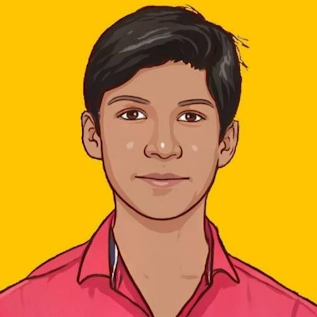
\includegraphics[width=3cm, height=3cm, keepaspectratio]{profile.jpg}};
    \end{tikzpicture}\\[1em]
    {\LARGE\bfseries\textcolor{primary}{Harshit Jaiswal}}\\[0.5em]
    \textcolor{primary}{\rule{0.4\textwidth}{0.5pt}}\\[1em]
    \textbf{Resume}
  \end{center}
}

\begin{document}

\maketitle

\section*{Contact Information}
\begin{tabularx}{\textwidth}{Xr}
    \textbf{Name:} & Harshit Jaiswal \\
    \textbf{Email:} & \href{mailto:harshitj183@gmail.com}{harshitj183@gmail.com} \\
    \textbf{Mobile:} & +91 9793009391 \\
    \textbf{LinkedIn:} & \href{https://www.linkedin.com/in/harshitj183/}{linkedin.com/in/harshitj183} \\
    \textbf{Website:} & \href{https://www.harshitj183.in}{harshitj183.in} \\
\end{tabularx}

\section*{Profile Summary}
Passionate B.Tech student specializing in Computer Science and Engineering, with expertise in programming, web development, SEO, and prompt engineering. Proficient in creating innovative solutions, optimizing web performance, and managing freelance projects. Dedicated to contributing to technology and enhancing user experiences.

\section*{Education}
\begin{tabularx}{\textwidth}{Xr}
    \textbf{B.Tech in Computer Science and Engineering} & KR Mangalam University, Haryana, Delhi NCR \\
    Expected Graduation: 2027 & \\
    \textbf{10th and 12th Grade (Science)} & S Tulsi Inter College, Rajapur, Chitrakoot, UP \\
    Graduated: 2022 & \\
\end{tabularx}

\section*{Skills}
\begin{multicols}{2}
    \begin{itemize}[label=--]
        \item \textbf{Programming Languages:} Python, JavaScript, C++
        \item \textbf{Web Technologies:} HTML, CSS, PWA
        \item \textbf{Tools \& Platforms:} Blogger, WordPress, Google Search Console, Canva, Cloudflare, Replit, GitHub, Google Cloud, Firebase
        \item \textbf{Special Skills:} SEO, Prompt Engineering, Web Development, Custom Search Engine Implementation
        \item \textbf{Soft Skills:} Problem-solving, Adaptability, Attention to detail, Time management, Continuous learning
    \end{itemize}
\end{multicols}

\section*{Experience}
\textbf{Freelancer} \\
Various Clients \\
\textit{2017 -- Present}
\begin{itemize}[label=--]
    \item Completed over 24 freelance projects in web development, including full-stack solutions and customizations.
    \item Managed client communications, delivered tailored solutions, and ensured high satisfaction levels.
\end{itemize}

\section*{Certifications}
\begin{tabularx}{\textwidth}{Xr}
    \textbf{Certificate of Participation in Round 1: The Mind Maze of Nestlé Leaders League - Genesis} & Unstop \\
    Issued: June 2024 & Credential ID: 0e955a1a-89e8-471e-b6f1-4a609cccc7ec \\
    \textbf{Introduction to Career Skills in Software Development} & LinkedIn \\
    Issued: June 2024 & \\
    \textbf{Programming Foundations: Fundamentals} & LinkedIn \\
    Issued: June 2024 & \\
    \textbf{Certificate of Participation in Samsung Galaxy AI Treasure Hunt} & Unstop \\
    Issued: May 2024 & Credential ID: 7ad266d3-bf16-4b91-8a34-a5d33744c000 \\
    \textbf{Certificate of Participation in Consultathon 4.0} & Unstop \\
    Issued: November 2023 & Credential ID: 82a34730-52f4-444c-ab73-f5ed9489a564 \\
\end{tabularx}

\section*{Personal Interests}
\begin{itemize}[label=--]
    \item Enjoy spending quality alone time, reading books, drawing, and listening to music and podcasts.
    \item Active user of Quora for knowledge sharing and learning.
\end{itemize}

\section*{Professional Goals}
Aiming to work as a freelancer with a focus on contributing to DRDO and ISRO in space research and software programming. Dedicated to leveraging skills to contribute significantly to technological advancements and national development.

% Signature (Optional)
\begin{center}
    
\includegraphics[width=5cm, height=2cm, keepaspectratio]{signature.jpg}
    \vspace{0.5cm}
    \textbf{Harshit Jaiswal} \\
    \textit{@harshitj183}
\end{center}

\end{document}
